\documentclass[mathserif]{beamer}
\mode<presentation>
{
  \usetheme{Frankfurt}
  \setbeamercovered{transparent}
}

\setbeamertemplate{caption}[numbered]

\usepackage{bm}
\usefonttheme[onlymath]{serif}
\usepackage{mathrsfs}

\begin{document}


\title{Trust Region Policy Optimization}

\author{Wenhao Yang
}
\institute{School of Mathematical Sciences

Peking University}
\begin{frame}
  \titlepage
\end{frame}

\date{}

\begin{frame}{Outline}
\tableofcontents
\end{frame}

\section{Preliminaries}
\begin{frame}[t]{Markov Decision Process}
\begin{itemize}
  \item Dynamic system: $(\mathcal{S},\mathcal{A},P,r,\rho_{0},\gamma)$
  \item $P:\mathcal{S}\times\mathcal{A}\times\mathcal{S}\rightarrow\mathbb{R}$
  \item $\rho_{0}:\mathcal{S}\rightarrow\mathbb{R}$
  \item $\pi:\mathcal{S}\times\mathcal{A}\rightarrow[0,1]$ is a stochastic policy
  \item $\eta(\pi)$ is expected discounted reward:
  \begin{align}
    \eta(\pi)=E_{s_{0},a_{0},...}[\sum_{t=0}^{\infty}\gamma^{t}r(s_{t})]
  \end{align}
  where $s_{0}\sim\rho_{0}(s_{0})$, $a_{t}\sim\pi(a_{t}|s_{t})$, $s_{t+1}\sim P(s_{t+1}|s_{t},a_{t})$
\end{itemize}
\end{frame}
\begin{frame}[t]{Actor-Critic Decomposition}
\begin{itemize}
  \item $Q_{\pi}(s_{t},a_{t})=E_{s_{t+1},a_{t+1},...}[\sum_{l=0}^{\infty}\gamma^{l}r(s_{t+l})]$
  \item $V_{\pi}(s_{t})=E_{a_{t},s_{t+1}...}[\sum_{l=0}^{\infty}\gamma^{l}r(s_{t+l})]$
  \item $A_{\pi}(s,a)=Q_{\pi}(s,a)-V_{\pi}(s)$
  \item $a_{t}\sim\pi(a_{t}|s_{t})$, $s_{t+1}\sim P(s_{t+1}|s_{t},a_{t})$
\end{itemize}
\begin{theorem}
  Given another policy $\tilde{\pi}$, the following equation holds:
  \begin{align}
    \eta(\tilde{\pi})=\eta(\pi)+E_{s_{0},a_{0},...\sim\tilde{\pi}}[\sum_{t=0}^{\infty}\gamma^{t}A_{\pi}(s_{t},a_{t})]
  \end{align}
\end{theorem}
\begin{itemize}
  \item Denote $\rho_{\pi}(s)=P(s_{0}=s)+\gamma P(s_{1}=s)+\gamma^{2}P(s_{2}=s)+...$ we have:
  \begin{align}
    \eta(\tilde{\pi})=\eta(\pi)+\sum_{s}\rho_{\tilde{\pi}}(s)\sum_{a}\tilde{\pi}(a|s)A_{\pi}(s,a)
  \end{align}
\end{itemize}
\end{frame}
\begin{frame}[t]{Actor-Critic Decomposition}
  \begin{itemize}
    \item The computation of $\rho_{\tilde{\pi}}$ is complex, which makes the equation(2) difficult to optimize directly.
    \item Approximation:
    \begin{align}
      L_{\pi}(\tilde{\pi})=\eta(\pi)+\sum_{s}\rho_{\pi}(s)\sum_{a}\tilde{\pi}(a|s)A_{\pi}(s,a)
    \end{align}
    \item If $\pi_{\theta}$ is a differential funtion of $\theta$, $L_{\pi}$ matches $\eta$ to first order
    \begin{align}
      L_{\pi_{\theta_{0}}}(\pi_{\theta_{0}})&=\eta{\pi_{\theta_{0}}}\\
      \nabla L_{\pi_{\theta_{0}}}(\pi_{\theta})_{|\theta=\theta_{0}}&=\nabla \eta(\pi_{\theta})|_{\theta=\theta_{0}}
    \end{align}
    \item Conservative policy iteration provide explicit lower bounds on the improvement of $\eta$.
  \end{itemize}
\end{frame}
\begin{frame}[t]{Conservative policy iteration}
  \begin{itemize}
    \item $\pi_{old}:$ the current policy
    \item $\pi'=\arg\max_{\pi'}L_{\pi_{old}}(\pi')$
    \item The new policy $\pi_{new}$ is defined as:
    \begin{align}
      \pi_{new}(a|s)=(1-\alpha)\pi_{old}(a|s)+\alpha\pi'(a|s)
    \end{align}
    \item Lower bound:
    \begin{align}
      \eta(\pi_{new})\ge L_{\pi_{old}}(\pi_{new})-\frac{2\varepsilon\gamma}{(1-\gamma)^{2}}\alpha^{2}
    \end{align}
    where $\varepsilon=\max_{s}|E_{a\sim\pi'(a|s)}[A_{\pi}(s,a)]|$
    \item This lower bound if unwieldy and restrictive in practice.
  \end{itemize}
\end{frame}

\section{Monotonic Improvement}
\begin{frame}[t]{Improvement}
\begin{itemize}
\item The bound can be extended to general stochastic policies by replacing $\alpha$ with a distance measure between $\pi$ and $\tilde{\pi}$ and changing the constant $\varepsilon$ appropriately.
\item Distance measure: $D_{TV}(p\parallel q)=\frac{1}{2}\sum_{i}|p_{i}-q_{i}|$
\item $D_{TV}^{\max}(\pi,\tilde{\pi})=\max_{s}D_{TV}(\pi(\cdot|s)\parallel\tilde{\pi}(\cdot|s))$
\end{itemize}
\begin{theorem}
Let $\alpha=D_{TV}^{\max}(\pi_{old},\pi_{new})$, then the following bound holds:
\begin{align}
  \eta(\pi_{new})\ge L_{\pi_{old}}(\pi_{new})-\frac{4\varepsilon\gamma}{(1-\gamma)^{2}}\alpha^{2}
\end{align}
where $\varepsilon=\max_{s,a}|A_{\pi}(s,a)|$
\end{theorem}
\end{frame}

\begin{frame}[t]{Improvement}
\begin{itemize}
  \item Note that $D_{TV}(p\parallel q)^{2}\le D_{KL}(p\parallel q)$, then the bound becomes as:
  \begin{align}
      \eta(\pi_{new})\ge L_{\pi_{old}}(\pi_{new})-\frac{4\varepsilon\gamma}{(1-\gamma)^{2}}D_{KL}^{\max}(\pi_{new},\pi_{old})
  \end{align}
  \item Algorithm:
  \begin{figure}
    \centering
    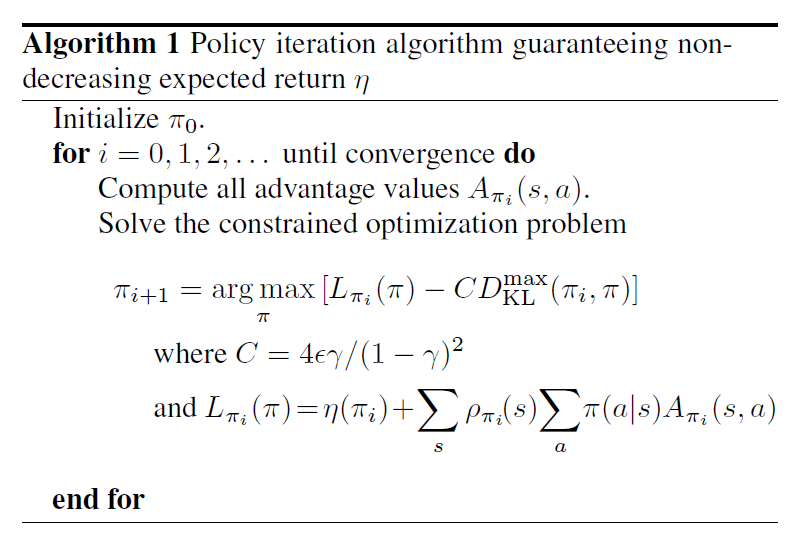
\includegraphics[scale=0.5]{fig/1}
  \end{figure}
\end{itemize}
\end{frame}

\begin{frame}[t]{Improvement}
\begin{itemize}
  \item This algorithm is guaranteed to generate a monotonically improving sequence of policies $\eta(\pi_{0})\le\eta(\pi_{1})\le\eta(\pi_{2})\le...$

  \item In fact, let $M_{i}(\pi)=L_{\pi_{i}}(\pi)-CD_{KL}^{\max}(\pi_{i},\pi)$, then:
  \begin{align}
    &\eta(\pi_{i+1})\ge M_{i}(\pi_{i+1})\\
    &\eta(\pi_{i})=M_{i}(\pi_{i})\\
    &\eta(\pi_{i+1})-\eta(\pi_{i})\ge M_{i}(\pi_{i+1})-M_{i}(\pi_{i})
  \end{align}

  \item Trust Region Policy Optimization is an approximation to this Algorithm.
\end{itemize}
\end{frame}

\section{Opt of Parameterized Policies}
\begin{frame}[t]{Trust Region Policy Optimization}
  \begin{itemize}
    \item Consider $\pi_{\theta}(a|s)$ as a function of parameter $\theta$, the algorithm is aim to optimize:
    \begin{align}
      \max_{\theta} L_{\theta_{old}}(\theta)-CD_{KL}^{\max}(\theta_{old},\theta)
    \end{align}
    \item Problem: Step size would be very small.
    \item To take larger steps in a robust way:
    \begin{align}
      &\max_{\theta}L_{\theta_{old}}(\theta)\\
      &s.t. \hspace{4pt}D_{KL}^{\max}(\theta_{old},\theta)\le\delta
    \end{align}
    \item Problem: Too many constrains.
    \item Do a heuristic approximation which considers the average KL divergence:
    \begin{align}
      \bar{D}_{KL}^{\rho_{old}}(\theta_{old},\theta)=E_{s\sim\rho_{0}}[D_{KL}(\pi_{\theta_{old}}(\cdot|s)\parallel\pi_{\theta}(\cdot|s))]\le\delta
    \end{align}
  \end{itemize}
\end{frame}

\section{Sample-Based Estimation}
\begin{frame}[t]{Approximation by MC}
  \begin{itemize}
    \item Optimization problem:
    \begin{align}
      \max_{\theta} &\sum_{s}\rho_{\theta_{old}}(s)\sum_{a}\pi_{\theta}(a|s)A_{\theta_{old}}(s,a)\\
      &s.t.\hspace{4pt}\bar{D}_{KL}^{\rho_{old}}(\theta_{old},\theta)\le\delta
    \end{align}
    \item Sample formation:
    \begin{align}
      &\max_{\theta}E_{s\sim\rho_{old},a\sim q}[\frac{\pi_{\theta}(a|s)}{q(a|s)}Q_{\theta_{old}}(s,a)]\\
      &s.t.\hspace{4pt}\bar{D}_{KL}^{\rho_{old}}(\theta_{old},\theta)\le\delta
    \end{align}
    \item How to sample: 1. Single Path; 2. Vine
    \item Single Path is just sampling $s_{0}\sim\rho_{0}$ and simulate a sequence by $\pi_{\theta_{old}}$. Hence, $q=\pi_{\theta_{old}}$, $Q_{\theta_{old}}(s,a)$ is computed at each step.
  \end{itemize}
\end{frame}
\begin{frame}[t]{Vine}
\begin{itemize}
  \item Like A3C. Explaination on black-board
  \item In small, finite action spaces, every possible action can be generated from a given state:
  \begin{align}
    L_{n}(\theta)=\sum_{k=1}^{K}\pi_{\theta}(a_{k}|s_{n})\hat{Q}(s_{n},a_{k})
  \end{align}
  where action space is $\mathcal{A}=\{a_{1},a_{2},...,a_{K}\}$
  \item In large or continuous action spaces:
  \begin{align}
    L_{n}(\theta)=\frac{\sum_{k=1}^{K}\frac{\pi_{\theta}(a_{n,k}|s_{n})}{\pi_{\theta_{old}}(a_{n,k}|s_{n})}\hat{Q}(s_{n},a_{n,k})}{\sum_{k=1}^{K}\frac{\pi_{\theta}(a_{n,k}|s_{n})}{\pi_{\theta_{old}}(a_{n,k}|s_{n})}}
  \end{align}
\end{itemize}
\end{frame}

\section{Practical Algorithm}
\begin{frame}[t]{Practical Algorithm}
\begin{itemize}
  \item 1. Use Single Path or Vine to collect a set of state-action pairs along with MC estimates of their Q-Values
  \item 2. By averaging over samples, construct object function and constraint region
  \item 3. Solve the optimization problem to update the policy's parameter.
\end{itemize}
\end{frame}

\section{Reference}
\begin{frame}{Reference}
  Reference:

  [1] John Schulman, Sergey Levine, Philipp Moritz, Michael I. Jordan, Pieter Abbeel; Trust Region Policy Optimization
\end{frame}
\end{document}
